\documentclass[pdftex, 12pt, oneside]{article}

\usepackage[paperwidth=8.27in, paperheight=11.69in]{geometry}
\usepackage{graphicx}
\usepackage[english]{babel}
\usepackage{enumerate}
\usepackage{float}
\usepackage{gensymb}
\usepackage{listings}
\usepackage{color}

\newcommand{\HRule}{\rule{\linewidth}{0.5mm}}

\definecolor{codegreen}{rgb}{0, 0.6, 0}
\definecolor{codegray}{rgb}{0.5, 0.5, 0.5}
\definecolor{codepurple}{rgb}{0.58, 0, 0.82}
\definecolor{backcolor}{rgb}{0.95, 0.95, 0.92}

\lstdefinestyle{mystyle}{
  backgroundcolor=\color{backcolor},
  commentstyle=\color{codegreen},
  keywordstyle=\color{magenta},
  numberstyle=\tiny\color{codegray},
  stringstyle=\color{codepurple},
  basicstyle=\footnotesize,
  breakatwhitespace=false,
  breaklines=true,
  captionpos=b,
  keepspaces=true,
  numbers=left,
  numbersep=5pt,
  showspaces=false,
  showstringspaces=false,
  showtabs=false,
  tabsize=2
}

\lstset{style=mystyle}

\begin{document}

\textbf{\large TUTORIAL ZKOSS - HI }
\\[1cm]
\textbf{Priyanto Tamami}\\
tamami.oka@gmail.com\\
github.com/tamami

\HRule

\section{PENDAHULUAN}

Dengan berkembangnya dunia internet sekarang ini, kebutuhan akan sebuah sistem informasi berbasis \textit{web} semakin banyak diperlukan. Dari kebutuhan hanya sekedar menampilkan informasi perusahaan, sampai kepada pengolahan data entry sehingga menghasilkan laporan-laporan yang dapat diakses melalui sebuah \textit{website}.

Perkembangan jumlah pengguna internet yang semakin meningkat, pun demikian dari sisi penyedianya, entah yang menawarkan jasa \textit{hosting}, jasa \textit{cloud}, sampai dengan jasa untuk membangun sebuah aplikasi web.

Perkembangan teknologi untuk membangun aplikasi web pun tidak kalah berkembang, banyak \textit{framework} bermunculan dalam beberapa bahasa pemrograman, yang salah satu tujuannya yaitu mempercepat waktu dalam membangun sebuah aplikasi berbasis web. ZKOSS adalah salah satunya.

\section{ISI}

\textit{Framework} ZKOSS ini memang bukan sepenuhnya gratis, ada lisensi berbayarnya juga untuk beberapa \textit{tools}, jadi pembahasan kali ini kita akan coba yang versi gratisnya saja, yaitu versi komunitas.

\textit{Framework} ini mengusung konsep pembangunan aplikasi dengan model MVVM (Model-View-ViewModel), walau secara kasar tidak akan terlihat bedanya dengan konsep MVC (Model-View-Controller), dan ZKOSS pun sebetulnya mampu mengimplementasikan konsep MVC yang sudah terkenal.

Langsung saja kita bahas bagaimana membangun sebuah aplikasi sederhana dengan ZKOSS, untuk mempermudah dalam manajemen pustakanya, maka akan kita gunakan maven. Berikut langkah-langkahnya :

\begin{enumerate}
  \item Periksa apakah maven sudah terpasang di komputer yang akan kita gunakan dengan mengetikan perintah berikut pada \textit{console}
  
  \begin{verbatim}
  $ mvn -version
  \end{verbatim}
  
sehingga akan muncul keterangan versi Maven yang telah terpasang, jika memang belum ada, silahkan memasangnya terlebih dahulu.

  \item Membuat kerangka kerja maven untuk aplikasi yang akan kita bangun, perintahnya cukup sederhana, yaitu dengan mengetikan kode berikut pada \textit{console}
  
  \begin{verbatim}
  $ mvn archetype:generate -DarchetypeCatalog=http://mavensync.zkoss.org/
  maven2/
  \end{verbatim}
  
sehingga muncul menu pilihan berikut :

\begin{figure}[H]
  \centering
  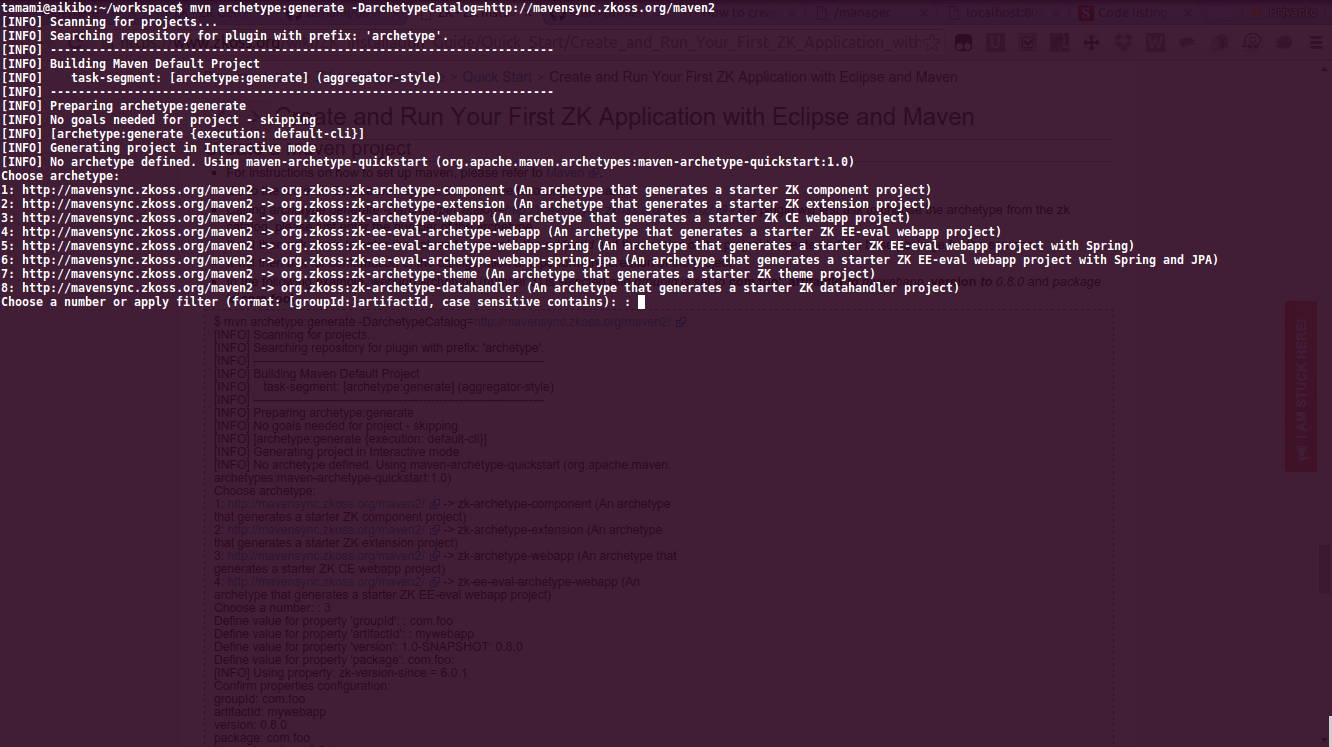
\includegraphics[width=0.7\textwidth]{./resources/pilihan-mvn-generate}
  \caption{Pilihan Dari Maven}
\end{figure}

Pilihan tersebut mungkin sama, mungkin juga berbeda, tergantung isi dari katalog yang ada pada http://mavensync.zkoss.org.

  \item Karena kita akan menggunakan aplikasi ini dengan gratis, maka ketikkan nomor yang menyebutkan pilihan ZK CE (Community Edition), atau kita bisa saja mencoba fasilitas \textit{trial} yang diberikan untuk versi berbayarnya. Dengan pilihan seperti pada Gambar 1, maka kita memilih nomor 3.
  
  Bila kita diminta untuk mengisikan \verb|groupId| atau \verb|artifactId|, isikan saja sembarang, yang biasanya, isian untuk \verb|groupId| seperti nama paket di Java, sebagai contoh lab.aikibo.tutorial, sedangkan \verb|artifactId| adalah nama \textit{project}-nya.
  
  Untuk pertanyaan berikutnya seperti \verb|version| dan \verb|package| cukup dilewat saja dengan menekan tombol Enter.
  
  \item Setelah selesai dengan membuat kerangka, maka akan terbentuk struktur \textit{folder} kerja yang nantinya kita gunakan.

\end{enumerate}

\section{PENUTUP}

\end{document}